\section{Background}

\subsection{Decision Tree}

A decision tree is a decision support tool that uses a tree-like graph or model of decisions and
their possible consequences. A diagram of decision tree structure is shown as Figure \ref{figure:decision_tree}. 

A decision tree is composed of decision nodes, start of the first decision (its root). There will be at least
two decision options after each judgement. Decisions are made by internal knowledge of agents, for example
parameters or constraints. 

At the beginning of a decision tree from the root, the tree will start to decide which option to make next
step by estimating current state value, and continues making decisions and choices at each node until it meets
a termination or there are no more decisions to make in this branch of tree. 

As it shown in Figure \ref{figure:decision_tree}. ‘Shell weight’ is the decision criterion which is incorporated in each
node until it reaches the termination or last state. 

\begin{figure}[htb]
    \centering
    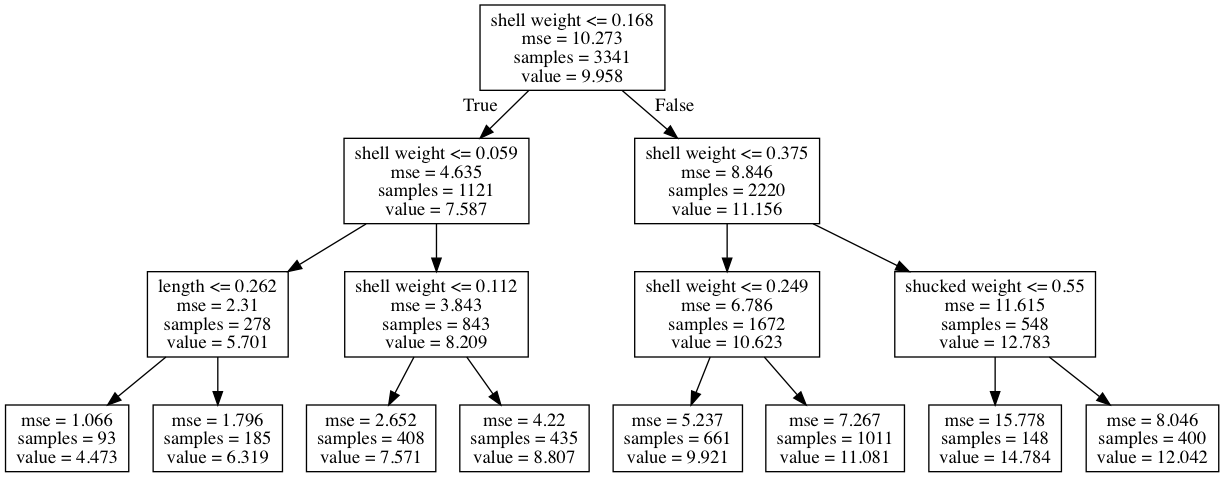
\includegraphics[width=1\textwidth]{images/decision_tree.png}
    \caption{Decision Tree}
    \label{figure:decision_tree}
\end{figure}

Decision tree can also control the behavior of the system in a simplifier way, by making decisions in script,
we can control the leaf node where the system will reach finally, as it shown in Figure \ref{figure:game_tree_search},
which is a decision tree of script applied to RTS game\cite{barriga2018game}, it controls the flow of the game
state: At the beginning game state will reach ‘Gather Resources’ leaf since that all game starts with one
defensive buildings. After gathering enough resources, which will lead to ‘Build defenses’ leaf, it starts to
‘Expand’ its base number. After enough bases was settled, the decision tree will lead the system to take some
offensive actions, first is to ‘Train Soldiers’. As we can see from Figure \ref{figure:game_tree_search}, according
to decision criterion, ‘Attack’ is final action that the game system will take.

\begin{figure}[htb]
    \centering
    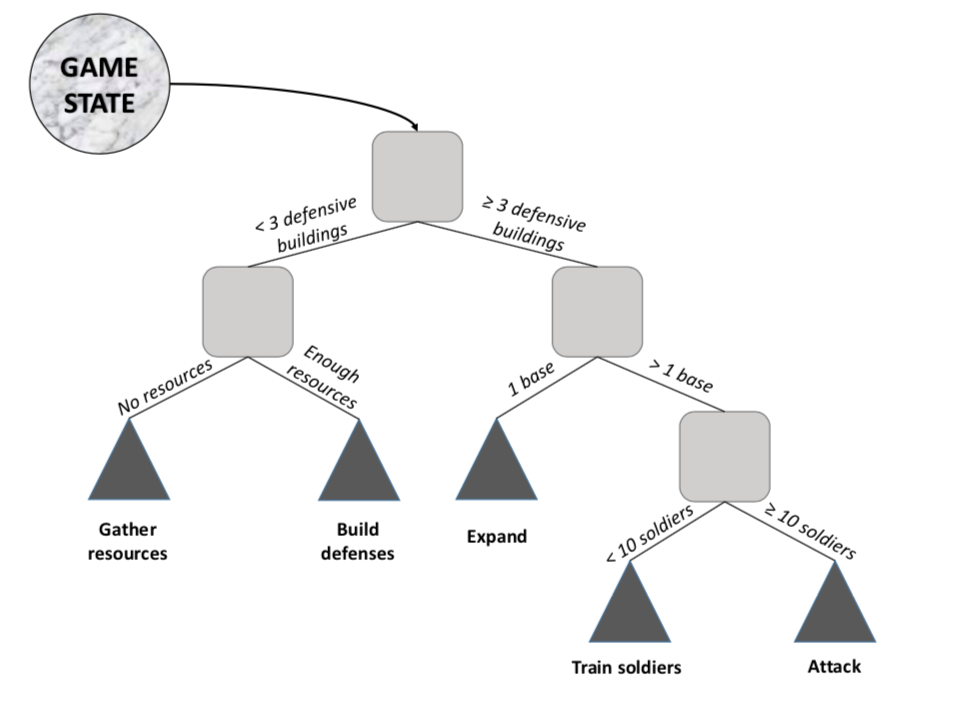
\includegraphics[width=0.7\textwidth]{images/game_tree_search.png}
    \caption{Game Tree Search\cite{barriga2018game}}
    \label{figure:game_tree_search}
\end{figure}

\subsection{Behavior Tree}

A behavior tree is a model of plan execution that is graphically represented as a tree\cite{marcotte2017behavior}.
A simple structure of Behavior Tree is shown as Figure \ref{figure:behavior_tree}. A Behavior Tree is a mathematical model,
which consists of actions and nodes. Behavior Trees can control the order and priority of actions by using different
types of nodes and can represent clearly a framework of a program. A Behavior Tree is often composed of 4 types of
typical nodes, all of them act different functions operating the tree. The four main types of nodes are illustrated
as below.

\subsubsection*{Composite Node}

Composite Node includes Selector Nodes, Sequence Nodes and Parallel Nodes. 

A Selector node will act as an OR operand when used in a Behavior Tree, when it begins, all child nodes of this Selector
node will be executed iteratively, if one of them is successfully executed, it will return a TRUE Boolean value, if not,
a False Boolean value will be returned and passed back to Selector node;

A Sequence Node can act as an AND operand when it is used in a Behavior Tree, when it begins, all child nodes of this
Sequence node will be executed iteratively, only if all child nodes are executed successfully, it will return a TRUE Boolean
value and passed it to Sequence Node;

Parallel Nodes provide a method to execute many nodes simultaneously. 

\subsubsection*{Decorator Node}

When Decorator Node is added in a Behavior Tree, it adds some extra actions to the return value received from its child
nodes and then pass the new value to the root.

\subsubsection*{Condition Node}

Act in Behavior Tree very simple, it will return a TRUE Boolean value only if the condition is satisfied, very similar to
nodes in a Decision Tree nothing but a Condition Node requires a return value.

\subsubsection*{Action Node}

Node that can specifically complete an action or a movement, an Action Node also requires return value.

\begin{figure}[htb]
    \centering
    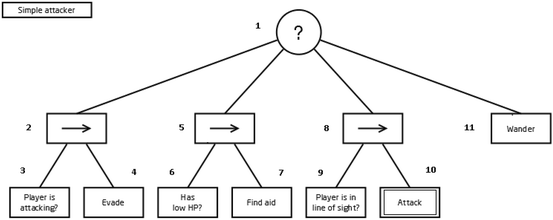
\includegraphics[width=0.9\textwidth]{images/behavior_tree.png}
    \caption{Behavior Tree\cite{marcotte2017behavior}}
    \label{figure:behavior_tree}
\end{figure}

\subsection{Breadth-First Search (BFS)}

Breadth-First Search is an algorithm that uses brute way to search all nodes first before it takes any action of exploring,
so it is an uninformed or blind algorithm of searching and does not know any goal information. 

Breadth-First Search is very simple, very easy to implement in algorithm but it requires lots of memory occupation since it
explores all nodes until find a termination or a goal.

\begin{figure}[htb]
    \centering
    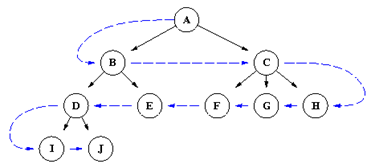
\includegraphics[width=0.5\textwidth]{images/BFS.png}
    \caption{BFS}
    \label{figure:BFS}
\end{figure}
